\begin{figure}[t]
  \centerline{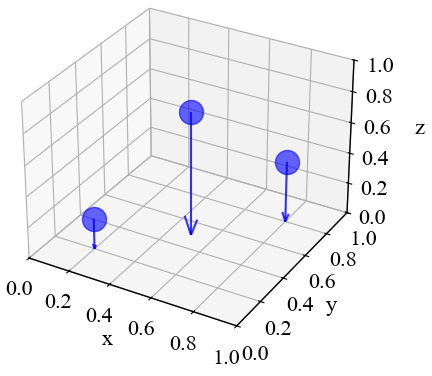
\includegraphics[width=\linewidth]{img/3d.png}}
  \caption{Projection of 3D coordinates}
  \label{trans3dto2d}
\end{figure}

Image-based feature modeling generates image arrays from time-series point-cloud frames and converts similarity changes between the arrays into statistics \cite{kizawa2023estimation}.
Overall physical movement is assumed to affect activity levels through changes in frame similarity.
\revised{Comparison of two point clouds requires point correspondence \cite{pomerleau2015review}.
Raw point-cloud frames do not provide the correspondence.
Frame-to-frame movement is not uniquely defined without the correspondence.
Orthogonal projection maps 3D occupancy onto a fixed 2D grid.}
For each frame, 3D point-cloud data are projected onto planes formed by pairs of the three coordinates ($x$, $y$, and $z$), as shown in Fig.~\ref{trans3dto2d}.
The projection is applied on all three axes for all frames.
Each 3D frame is converted into a 2D image to form a time-series 2D pixel array referred to as a `video frame'.
Frame-to-frame similarity is measured using zero-mean normalized cross-correlation (ZNCC) \cite{chen2020self,NAKHMANI2013315}.
ZNCC is computed between consecutive frames for the 1st to $I-1$-th frames, where $I$ is the number of frames.
The 50th and 90th percentile values of the ZNCC distribution are extracted as numerical features.
The 50th percentile value reflects the central tendency of the ZNCC distribution with minimal outlier influence.
The 90th percentile value captures upper-range similarity changes not represented by the central tendency alone.

Centroid feature modeling converts a head region of time-series point-cloud data into statistics of center-of-gravity changes.
Head movement is assumed to affect activity levels through center-of-gravity changes.
A head region is defined from 3D coordinates in an initial frame and extracted from all frames.
The sum of each coordinate in the head region is calculated for each frame.
Each frame is represented as a set of $n$ points ($x_{i}$, $y_{i}$, $z_{i}$) in 3D coordinate space.
The coordinate sums are defined as $X=\sum_{i=1}^{n}x_{i}$, $Y=\sum_{i=1}^{n}y_{i}$, and $Z=\sum_{i=1}^{n}z_{i}$.
The center of gravity $G_{j}$ for each frame up to $I$ is $G_{j}=(X/n, Y/n, Z/n)$, where $j$ is the frame number from the 1st to the $I$-th frame.
The central point $C$ of the center of gravity of all frames is $C=\frac{1}{I}\sum_{j=1}^{I}G_{j}$.
The difference between $C$ and $G_{j}$ is represented as Euclidean distance \cite{blais1995registering}.
The 50th and 90th percentile values of the center-of-gravity difference distribution are extracted as numerical features.
